\documentclass[11pt]{article}

\usepackage[margin=1in]{geometry}
\usepackage[T1]{fontenc}
\usepackage{graphicx}
\usepackage{amsmath}
\usepackage{float}
\usepackage{hyperref}

\hypersetup{
    colorlinks=true,
    linkcolor=blue,
    urlcolor=blue
}

\title{Histomics Causal Discovery and Multi-Omic Regulatory Graphs}
\author{Dylan Setiawan}
\date{Spring 2026}

\begin{document}
\maketitle

The initial goal of the project was to use single-cell histomics data to understand how local histone modifications around a gene interact with each other, and how those interactions might influence gene expression.
Instead of only asking whether one histone mark is present near a gene, I wanted to investigate whether multiple marks form a local regulatory structure together.
We wanted to ask whether promoter marks, enhancer-associated marks, and repressive marks appear coordinated around genes of interest using causal discovery.

The first major challenge was getting the data into a form where that question could even be asked.
The histone-mark datasets and the RNA data were not measured in the same feature space as they were derived from separate single-cell experiments, so we needed a way to integrate them. 
Jianle and I compared multiple integration methods and landed on scGLUE because it gave us the best integration results while still using a biologically meaningful guidance graph, graph neural network components, and a VAE-style latent representation.

\begin{figure}[H]
    \centering
    \begin{minipage}{0.49\textwidth}
        \centering
        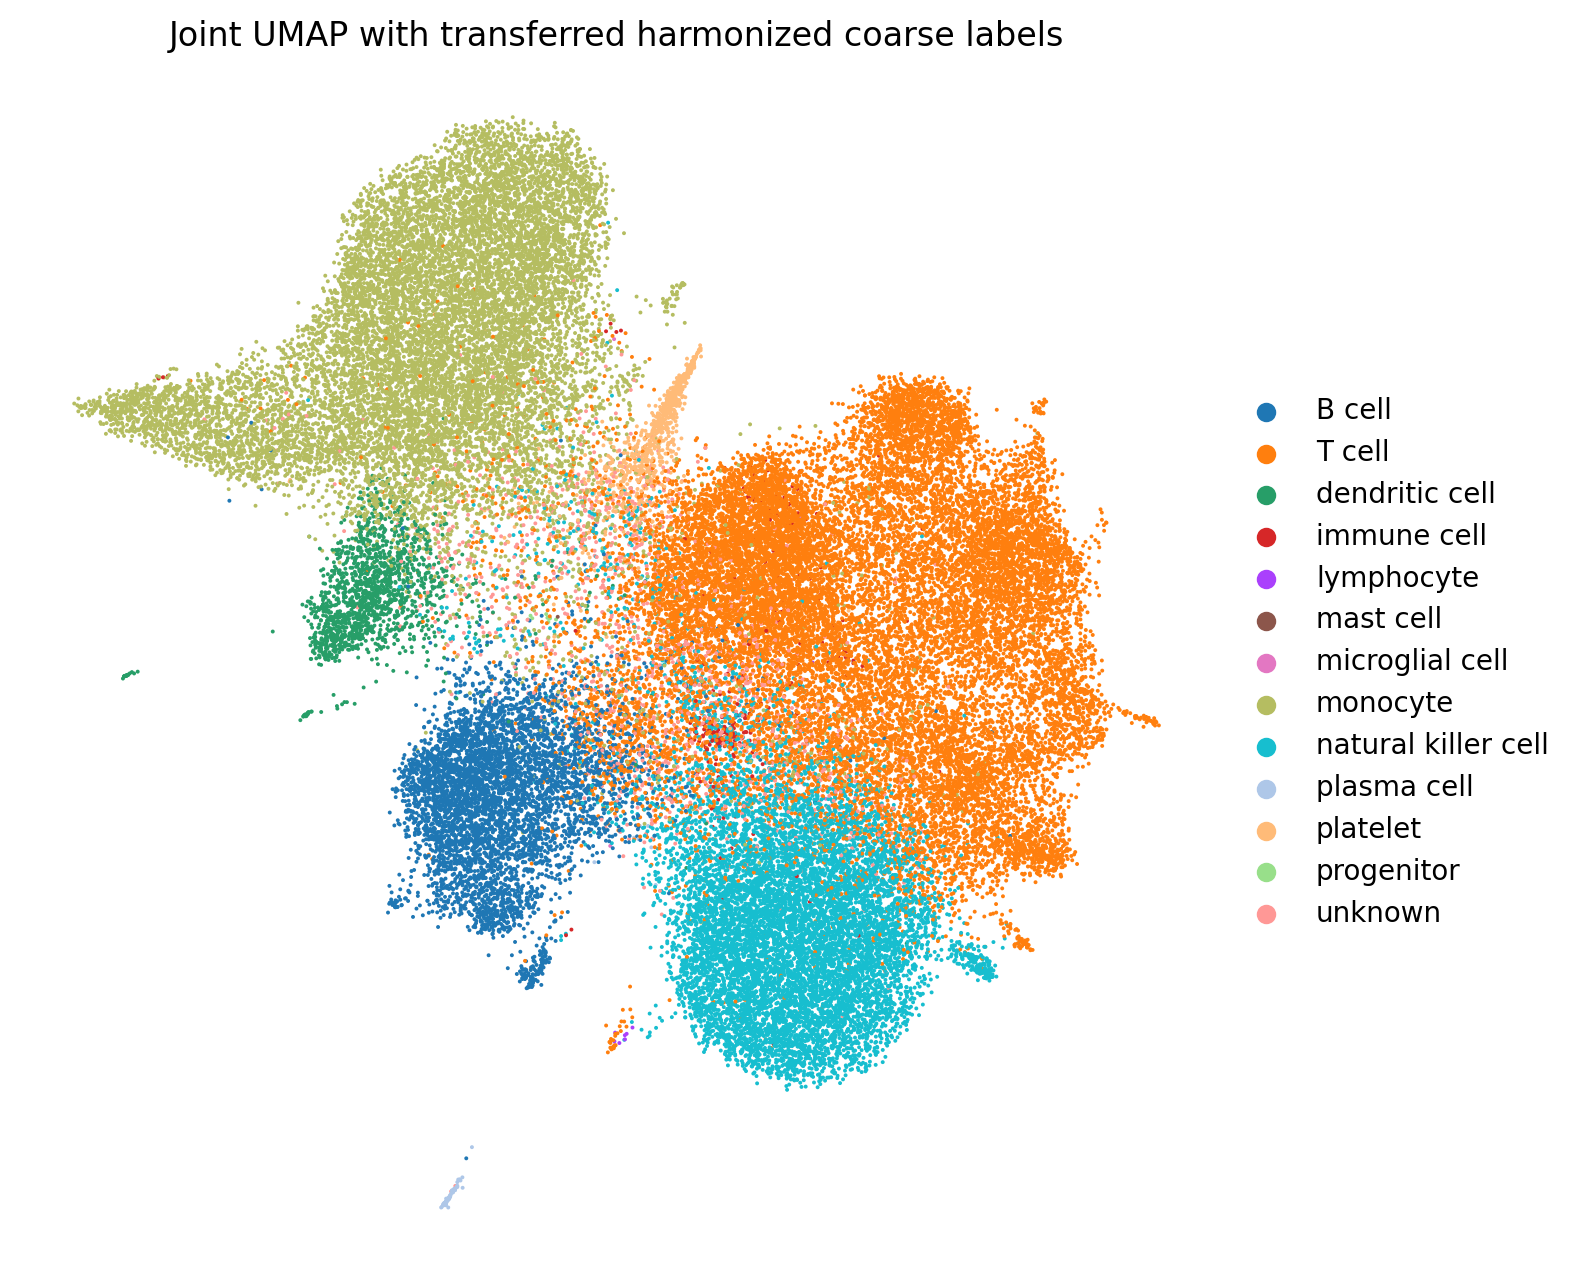
\includegraphics[width=\textwidth]{figures/umap_joint_harmonized_coarse.png}
    \end{minipage}
    \hfill
    \begin{minipage}{0.49\textwidth}
        \centering
        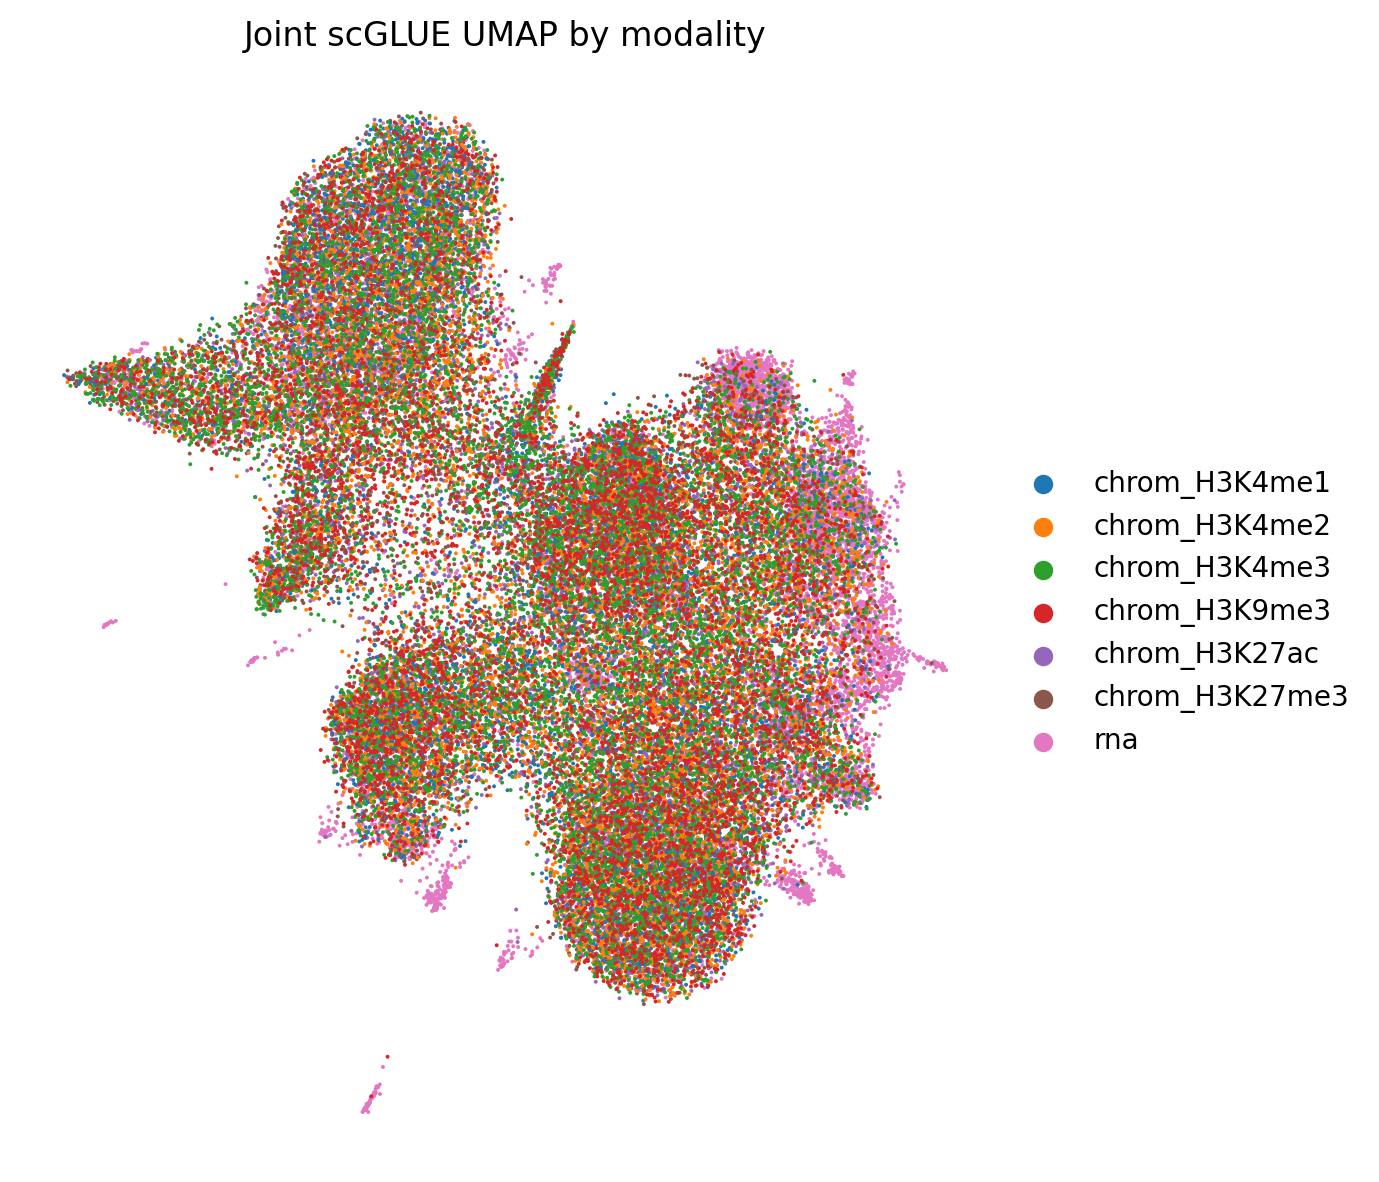
\includegraphics[width=\textwidth]{figures/umap_by_modality.png}
    \end{minipage}
    \caption{Joint scGLUE UMAPs colored by harmonized cell type (left) and modality (right).
    These plots show the shared space used to compare RNA and histone-mark modalities before constructing local graph inputs.}
    \label{fig:joint-umaps}
\end{figure}

With integration planned, we had a structured method to pair the cells together using the joint embedding and create the dataset for graph learning.
For each modality, we first cleaned and processed the data, used scGLUE to align the RNA and histone information, then built local gene-centered matrices for graph discovery.
We tried different graph-learning setups, different distributional assumptions for the nodes, different numbers of nearby peaks, and different ways of constraining or filtering the graph.

In the end, we were able to construct and validate graphs generated by multiple causal discovery algorithms (We tested PC, FCI, DAGMA). 
Through the results still require refinement, it has shown to be quite promising. 
Multiple nodes in the graphs have shown to map to enhancers and promoter regions in the literature. 
Moreover, paired scATAC-seq and RNA-seq were also analyzed in a similar manner to the histone data, and showed potential to be futher integrated into our current dataset.
So far, there does not seem to be a lot of research in peak to peak or enhancer to enhancer interactions suggesting that these results could provide a meaningful contribution in shedding the light on regulatory element dynamics within the local regulatory region of a gene.

\begin{figure}[H]
    \centering
    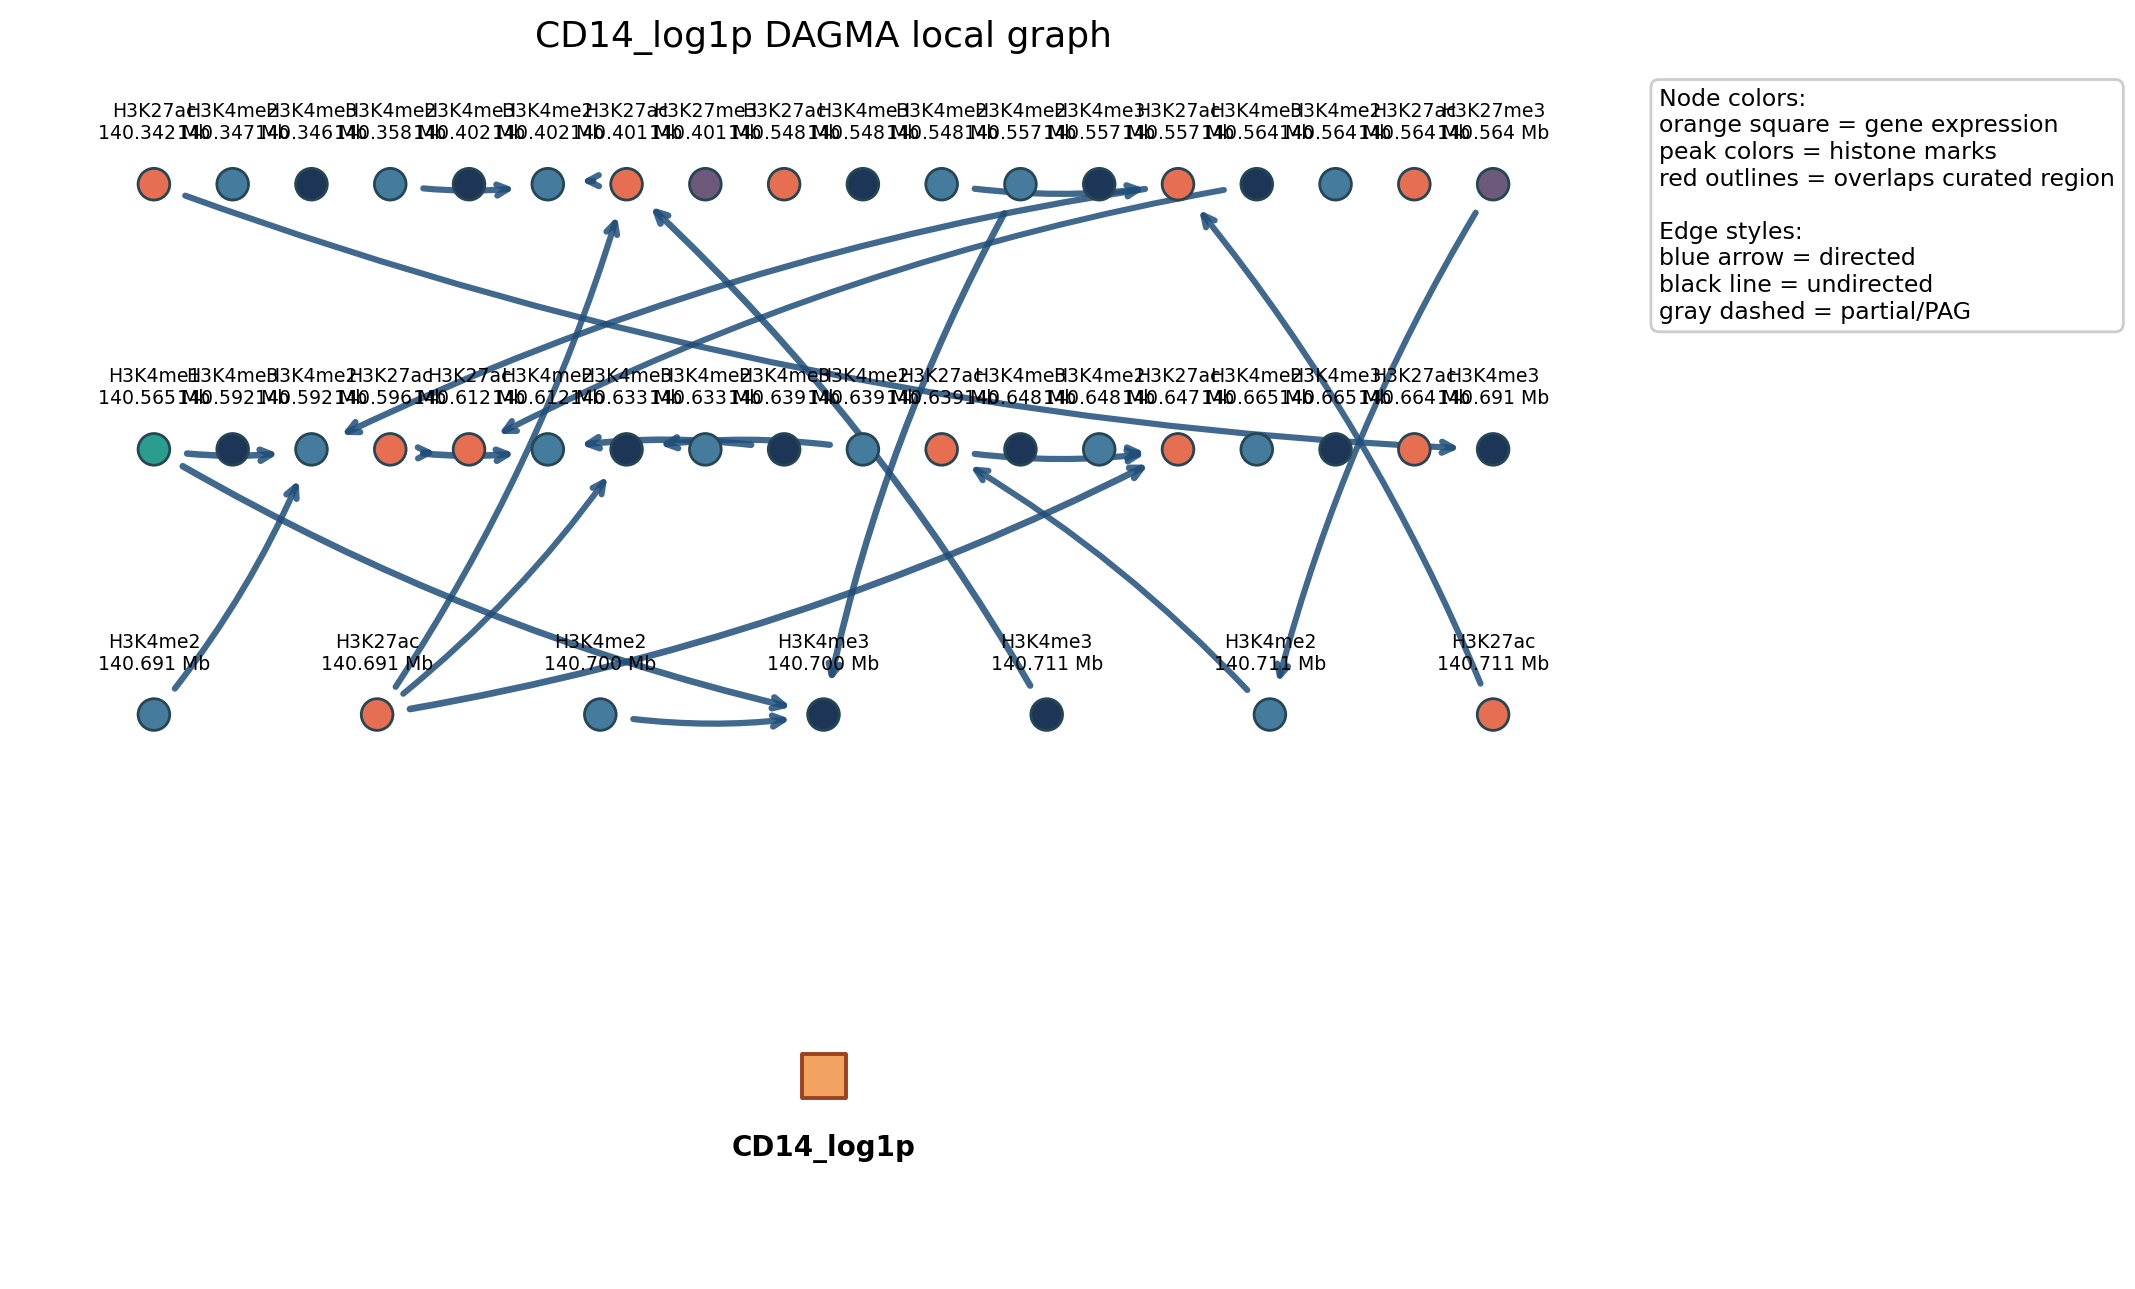
\includegraphics[width=0.9\textwidth]{figures/cd14_dagma_graph.png}
    \caption{CD14 histomics graph from nearby scCUT\&Tag peak features.
    A graph showing the potential coordination between histone marks for CD14, a well studied monocyte-relevant gene.}
    \label{fig:cd14-dagma}
\end{figure}

\begin{figure}[H]
    \centering
    \begin{minipage}{0.49\textwidth}
        \centering
        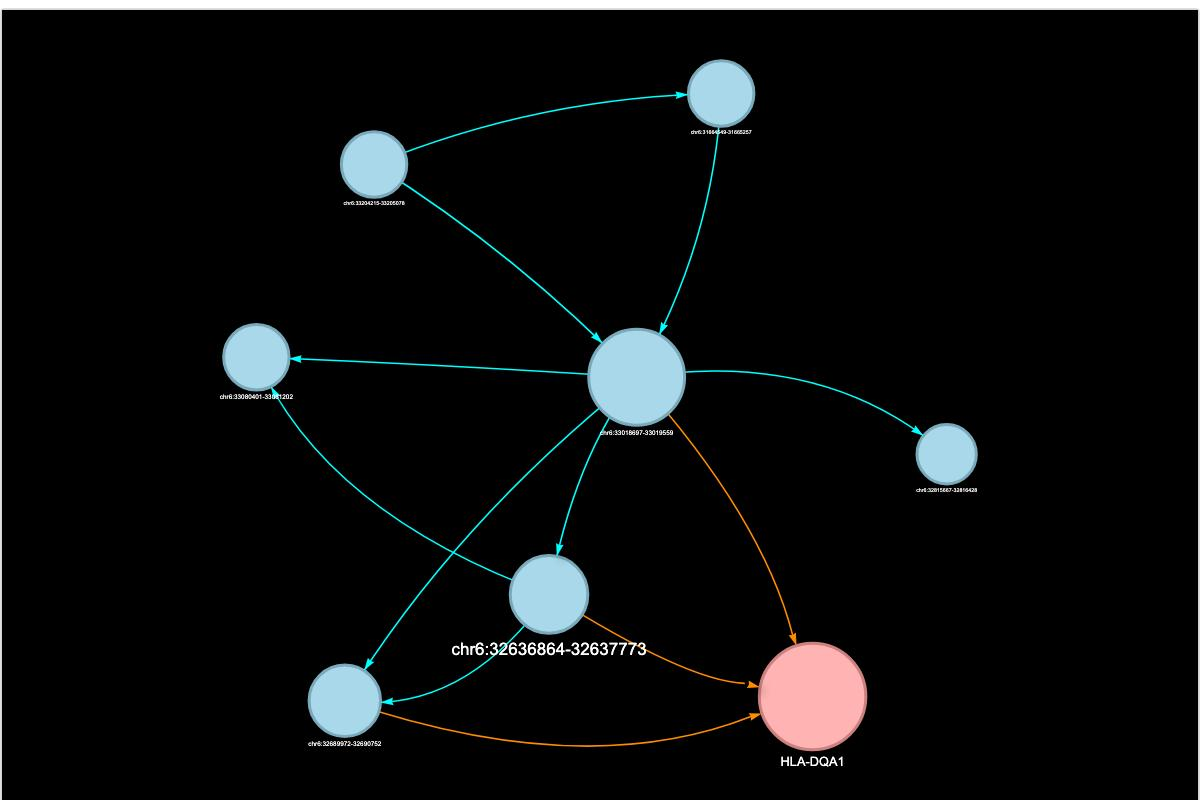
\includegraphics[width=\textwidth]{figures/hladqa1_atac_graph.jpeg}
    \end{minipage}
    \hfill
    \begin{minipage}{0.49\textwidth}
        \centering
        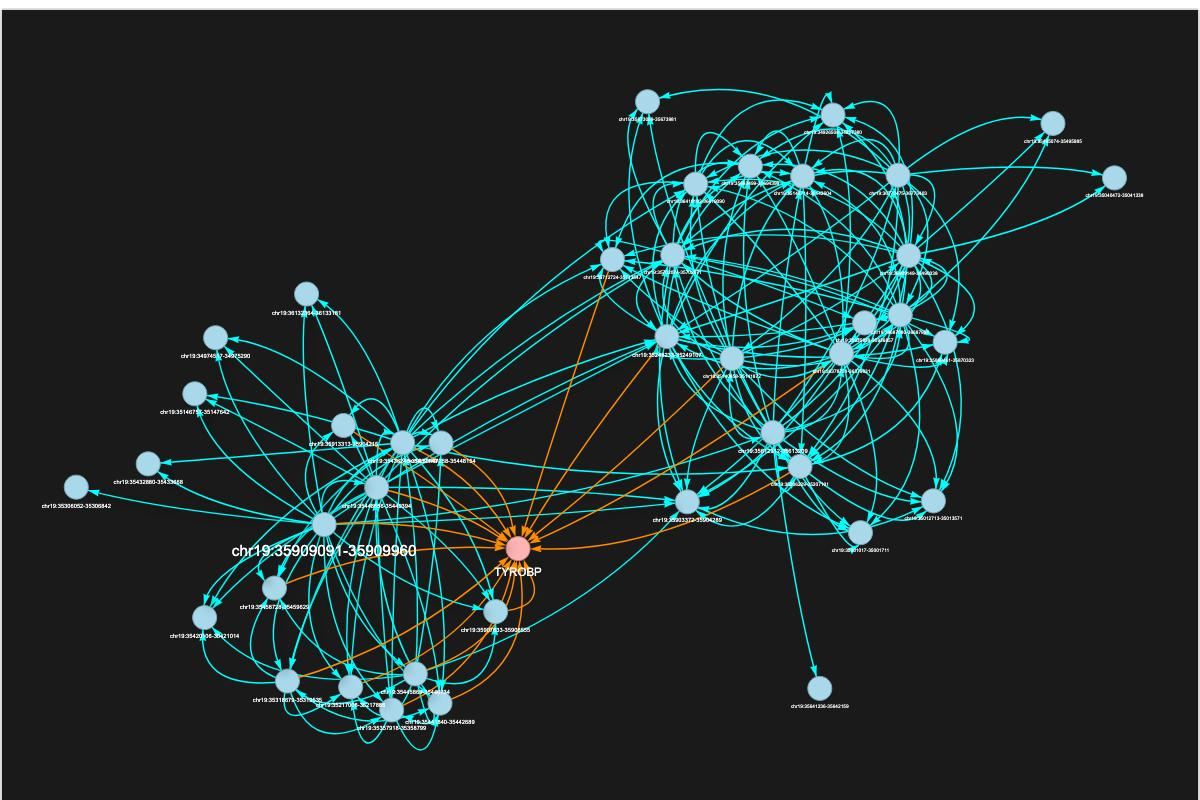
\includegraphics[width=\textwidth]{figures/tyrobp_atac_graph.jpeg}
    \end{minipage}
    \caption{Local ATAC-RNA graphs for HLA-DQA1 (left) and TYROBP (right).
    Multi-ome paired ATAC-seq and RNA-seq graphs showing peak to peak interactions and peak to gene interactions with metadata information as confounders.}
    \label{fig:atac-graphs}
\end{figure}

As our validation steps, we measured whether edges are stable throughout different graph learning configurations and different graph construction methods. 
Both datasets show extremely promising evidence with biological interpretation. An example being HLA-DQA1 being a gene that only acts in a specific cell type having a smaller regulatory neighborhood whilst TYROBP acts in multiple cell types and is backed by literature to have and need multiple pathways to activate as an immune response gene reflecting the complex network in the graph discovery process.

I believe that our current challenges are still rooted in the data complexity with how fragile integration is and how sparse the dataset is.
Jianle and I have discussed about how to proceed and have decided on these next steps:
\begin{itemize}
    \item Pairing cells using the average of nearby cells instead of a one to one pairing using the joint embedding (to fix the sparsity issue).
    \item Exploring the use of causal dropout when doing the graph learning.
    \item Increasing our local neighborhood window size to include more peaks and filter later (QC filtering or Elastic-net regularization).
    \item Increasing the robustness of our validations methods to not only include the Encode database, but also using JASPAR (TF-motif database) and potentially perturbation sequencing data. 
\end{itemize}

\end{document}
